\documentclass[12pt,letterpaper]{article}
\usepackage[utf8]{inputenc}
\usepackage{amsmath}
\usepackage{amsfonts}
\usepackage{amssymb}
\usepackage{cancel}
\usepackage[hmargin=2cm,vmargin=2cm]{geometry}
\usepackage{graphicx}
\usepackage{setspace}

\newcommand{\proofend}{\mbox{ }\hfill$\Box$\\}
\newcommand{\pdf}[2]{\frac{\partial #1}{\partial #2}}
\newcommand{\ddf}[2]{\frac{\mathrm{d} #1}{\mathrm{d} #2}}
\newcommand{\ee}[1]{\cdot10^{#1}}

\doublespacing

\begin{document}

{
\centering
\part*{An Electron Dispersion Compensator}
\section*{A Dispersion Compensator for Ultrafast Electron Pulses}
\section*{Untimed Pulse Compression For Electron Dispersion}
\section*{Untimed Dispersion Compensation for Ultrafast Electron Pulses}

\subsection*{Peter Hansen, Cory Baumgarten, Herman Batelaan, Martin Centurion\\
University of Nebraska-Lincoln\\
Department of Physics and Astronomy, Lincoln NE 68588\\
Email: mcenturion2@unlnotes.unl.edu}
}

\begin{abstract}
   PACS nrs.: 03.65.Ta, 03.75.-b, 03.65.Vf
\end{abstract}

   \section{Introduction}

Ultrafast Electron Microscopy (UEM) and Ultrafast Electron Diffraction (UED) are techniques that are used to study the dynamics of molecular motion. To do this short electron pulses are used to ``stroboscopically'' illuminate the molecules. However, electron pulse durations are limited to about 100 fs, while molecular dynamics extends into the low femto-second regime. Additionally, electronic motion can currently only be investigate directly with recollision approaches. A technique to deliver very short electron pulses on a target may extend UEM and UED into a regime that allows all molecular motion to be studied, and may allow the study of electronic motion of arbitrary targets.

Pulsed electron sources with pulse durations below 100 fs \cite{Bat} and even at sub-cycle duration (2.7 fs at 800 nm) have been reported \cite{Kasevich,Hommelhof}.  For these electron sources, the pulse has an appreciable energy spread of typically about 1 eV independent of energy. At a useful energy for UEM (100 keV) this means that the arrival time spread at a target 1 cm away from the source is a few microseconds even with a point source pulse. It is clear that a technique is required that reduces the temporal spread. Proposals for temporal lenses call for pulsed laser beams \cite{PNAS} or pulsed RF cavities \cite{Kraus} to affect the velocity of the electrons so that they regroup at the target. In this paper, we discuss an alternative idea to overcome the problem. We borrow an idea from optics, an optical dispersion compensator, and propose to use magnetic fields and a Wien filter to construct an  electron dispersion compensator. The differences between our electron dispersion compensator and these other proposed solutions which are all time dependent, is that the electron dispersion compensator is static, so like the optical dispersion compensator, it does not have to be synchronized with the electron pulses. A drawback is that this system can at best produce a pulse width as short as the one we start with, however current electron sources, as shown above, produce pulse widths well into the regime beneficial for UED and UEM and this technique will continue to apply as [sources get better].

Optics first then electrions. go element by element 1st grating 1st bfield, 2nd grating/2nd bfield $\rightarrow$ parallel pathsspread by velocity.

The electron dispersion compensator is modelled after the optical dispersion compensator.  The dispersive element is a pair of magnetic fields which disperse the electrons according to velocity, similarly to the angled gratings in an optical compensator which disperse light according to wavelength. The time spent in these magnetic fields is independent of velocity so they do not contribute any delay. The compensation $\Delta t$ in the optical compensator depends only on the path length difference $\Delta l$, so $\Delta t=\frac{\Delta l}{c}$ where $c$ is the speed of light. For electrons $\Delta t$ depends on a velocity change $\Delta v$, so $\Delta t = \frac{l}{\Delta v}$ where $l$ is the path length. We use a Wien Filter, a pair of crossed magnetic and electric fields. The electric field sets up a linear potential which slows down the higher energy electrons and speed up the lower energy electrons. 
The difference between the optical dispersion in a vacuum and electron dispersion is the dispersion relationship, given by \eqref{eq:disp}. The group velocity of light in a vacuum $v_{g \gamma}$ is equal to the phase velocity $v_{p\gamma}$, but for particles, $v_{ge}=2 v_{pe}$. 
\begin{align}
   \label{eq:disp}
E_\gamma=p_\gamma c &\qquad E_e=\frac{p_e^2}{2m}\\ 
w_\gamma =k_\gamma c &\qquad  w_e =\frac{\hbar^2 k_e^2}{2m} \\
v_{p\gamma} =c \quad v_{g\gamma}=c &\qquad  v_{pe} = \frac{\hbar^2 k_e}{2m} \quad v_{ge} = \frac{\hbar^2 k_e}{m}
\end{align}

\begin{figure}[htb]
   \centering
   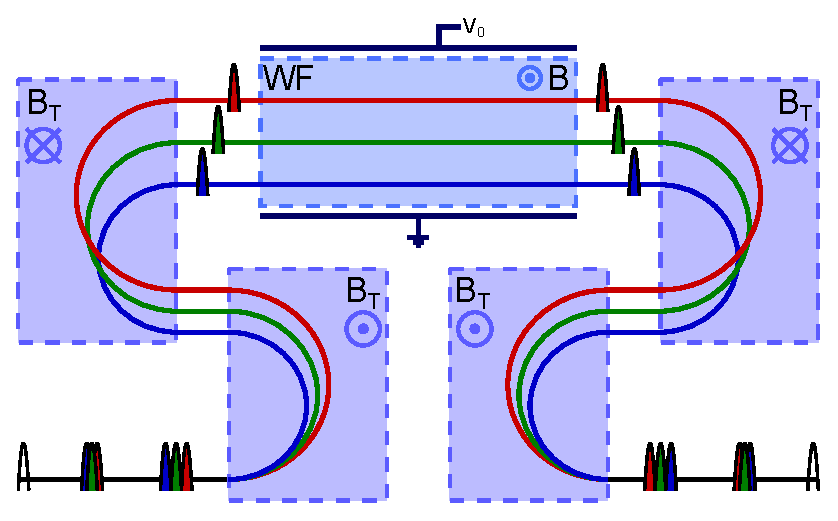
\includegraphics{Setup}
   \caption{Setup of the Electron Dispersion Compensator}
   \label{fig:setup}
\end{figure}
%\begin{figure}[htb]
%   \centering
%   \includegraphics{}
%   \caption{Setup of the Electron Dispersion Compensator}
%   \label{fig:setup}
%\end{figure}

\subsection{Theory}


\section{Simulation}

\section{Conclusion}
\end{document}

